\begin{mydefs}
	\iftoggle{eleve}{%
		La mesure \hrulefill
		
		\vspace*{0.2cm}
		\hrulefill 
		
		La longueur \hrulefill
		
	}{%
	La mesure d'un segment (distance entre ses deux extrémités) est sa \kw{longueur}.
	
	La longueur d'un segment $[AB]$, se note $AB$ ou $BA$. 
}
\end{mydefs}


\begin{myex}
	\vspace*{-0.5cm}
	\begin{center}
		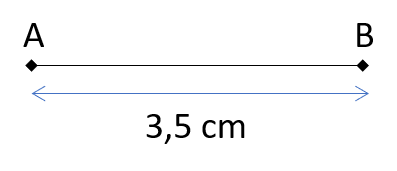
\includegraphics[scale=0.8]{img/lgr}
	\end{center}
	\vspace*{-0.5cm}
	
	\iftoggle{eleve}{%
		La longueur \hrulefill
		\vspace*{0.2cm}
		\hrulefill 
}{%
	La longueur du segment $[AB]$ est de \num{3.5} cm, on note $AB=\num{3.5}$ cm.
}	
	
\end{myex}

\begin{mydef}
	\iftoggle{eleve}{%
		Le \kw{milieu} d'un segment \hrulefill \\
		\vspace*{0.2cm}
		\hrulefill 
	}{%
		Le \kw{milieu} d'un segment est le point qui appartient au segment \kw{et} qui est à égale distance de ses extrémités.
	}
	
\end{mydef}

\begin{myrem}
	\iftoggle{eleve}{%
		Des segments de \hrulefill 
		
		\vspace*{0.2cm}
		\hrulefill 
	}{%
		Des segments de même longueur sont codés de façon identique.
	}
	
\end{myrem}

\begin{myex}
	
	\begin{center}
		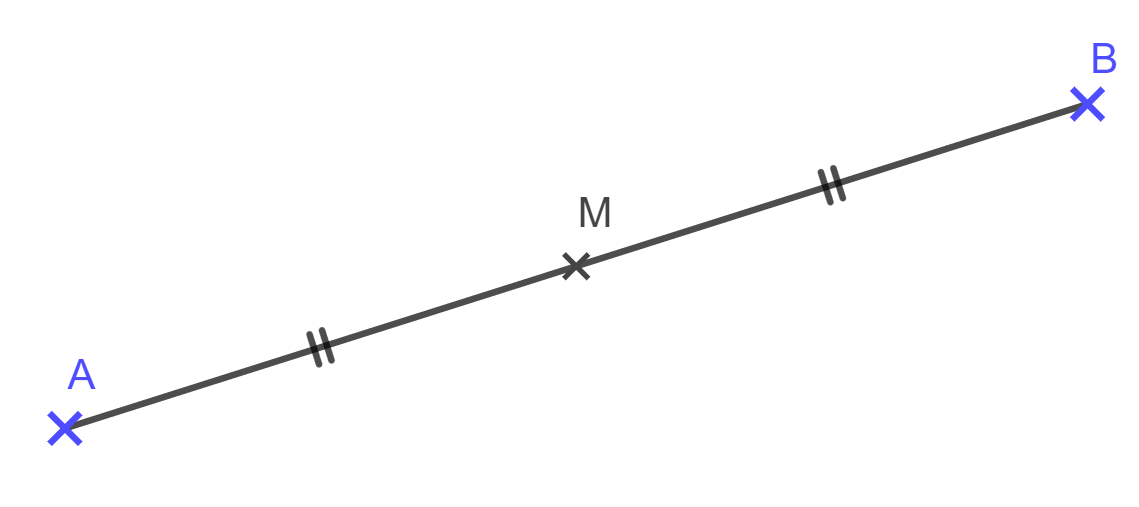
\includegraphics[scale=0.35]{img/milieu}
	\end{center}
	\iftoggle{eleve}{%
		On a : $M \in [AB]$ \hrulefill 
		
		\vspace*{0.2cm}
		\hrulefill 
	}{%
		On a : $M \in [AB]$ et $AM = MB$, donc le point $M$ est le milieu du segment $[AB]$. On a ainsi $AM = AB \div 2$. 
	}

\end{myex}

 \newpage

\begin{mydef}
	La distance d’un point à une droite est la longueur du plus court chemin entre ce point et la droite.
\end{mydef}

\begin{myprop}
	La distance d’un point $A$ à une droite $(d)$ est la longueur du segment $[AH]$, avec $H$ le pied de la perpendiculaire à $(d)$ passant par $A$.
\end{myprop}

\begin{center}
	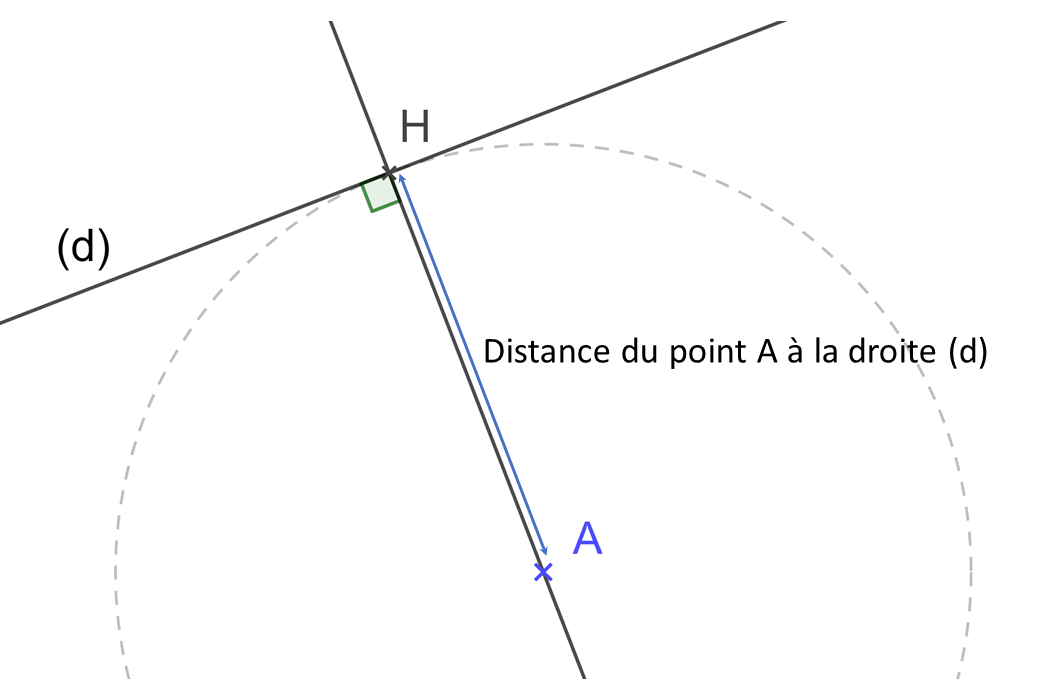
\includegraphics[scale=0.5]{img/lgr_droite}
\end{center}